Στην εργασία αυτή βασίστηκα σε κώδικα ο οποίος είχε αναπτυχθεί για την εργασία Efficient Byzantine Fault Tolerance \cite{minbftsystem}. Στην εργασία αυτή είχε αναπτυχθεί ο κώδικας για τον αλγόριθμο MinBFT, που αναφέραμε στην  ενότητα \ref{minbftSection}. Το MinBFT για την λειτουργία του χρησιμοποιεί το interface USIG (βλ. ενότητα \ref{usigSection}). Στην δουλεία εκείνη για την ανάπτυξη του USIG χρησιμοποιήθηκε η τεχνολογία Trusted Platform Module (TPM).

Υπενθυμίζουμε ότι ένα blockchain απαιτεί ένα μηχανισμό για την επίτευξη κατανεμημένης συμφωνίας ή την επικύρωση και την κανονικοποίηση ενός μόνο καταλόγου. Το πρωτόκολλο BFT αναφέρεται στο χαρακτηριστικό των κατανεμημένων συστημάτων που τους επιτρέπει να φτάσουν σε συμφωνία ενάντια στα βυζαντινά σφάλματα, δηλαδή σε καταστάσεις όπου τα συστατικά του συστήματος θα αποτύχουν - αλλά όχι μόνο να αποτύχουν - οι εσφαλμένοι βυζαντινοί κόμβοι θα ενεργήσουν αυθαίρετα και συχνά παρουσιάζουν αντικρουόμενες πληροφορίες σε διαφορετικούς κόμβους του συστήματος.

Υπενθυμίζουμε ότι ένα blockchain απαιτεί ένα μηχανισμό για την επίτευξη κατανεμημένης συμφωνίας ή την επικύρωση και την κανονικοποίηση ενός μόνο καταλόγου. Το πρωτόκολλο BFT αναφέρεται στο χαρακτηριστικό των κατανεμημένων συστημάτων που τους επιτρέπει να φτάσουν σε συμφωνία ενάντια στα βυζαντινά σφάλματα, δηλαδή σε καταστάσεις όπου τα συστατικά του συστήματος θα αποτύχουν - αλλά όχι μόνο να αποτύχουν - οι εσφαλμένοι βυζαντινοί κόμβοι θα ενεργήσουν αυθαίρετα και συχνά παρουσιάζουν αντικρουόμενες πληροφορίες σε διαφορετικούς κόμβους του συστήματος.

Υπενθυμίζουμε ότι ένα blockchain απαιτεί ένα μηχανισμό για την επίτευξη κατανεμημένης συμφωνίας ή την επικύρωση και την κανονικοποίηση ενός μόνο καταλόγου. Το πρωτόκολλο BFT αναφέρεται στο χαρακτηριστικό των κατανεμημένων συστημάτων που τους επιτρέπει να φτάσουν σε συμφωνία ενάντια στα βυζαντινά σφάλματα, δηλαδή σε καταστάσεις όπου τα συστατικά του συστήματος θα αποτύχουν - αλλά όχι μόνο να αποτύχουν - οι εσφαλμένοι βυζαντινοί κόμβοι θα ενεργήσουν αυθαίρετα και συχνά παρουσιάζουν αντικρουόμενες πληροφορίες σε διαφορετικούς κόμβους του συστήματος.

\section{Ενεργοποιώντας το Intel SGX}
Η τεχνολογία Intel SGX στους υπολογιστές από προεπιλογή είναι απενεργοποιημένη. Για να χρησιμοποιήσει κανείς το Intel SGX πρέπει να το ενεργοποιήσει αρχικά μέσω του BIOS. Αυτό απαιτεί ένα BIOS όπου από τον κατασκευαστή του υποστηρίζει ρητά το Intel SGX. Η υποστήριξη που παρέχεται από το BIOS μπορεί να ποικίλει μεταξύ κατασκευαστών. Για να λειτουργήσει το Intel SGX, αφού ενεργοποιήσουμε στο BIOS, πρέπει να εγκατασταθεί στο σύστημα το πακέτο λογισμικού Intel SGX Platform (ή αλλιώς PSW)\cite{linuxsgx}. 

Η τεχνολογία Intel SGX στους υπολογιστές από προεπιλογή είναι απενεργοποιημένη. Για να χρησιμοποιήσει κανείς το Intel SGX πρέπει να το ενεργοποιήσει αρχικά μέσω του BIOS. Αυτό απαιτεί ένα BIOS όπου από τον κατασκευαστή του υποστηρίζει ρητά το Intel SGX. Η υποστήριξη που παρέχεται από το BIOS μπορεί να ποικίλει μεταξύ κατασκευαστών. Για να λειτουργήσει το Intel SGX, αφού ενεργοποιήσουμε στο BIOS, πρέπει να εγκατασταθεί στο σύστημα το πακέτο λογισμικού Intel SGX Platform (ή αλλιώς PSW)\cite{linuxsgx}. 

\section{Trusted Monotonic Counter} \label{monotonicCounterimpl}
Η τεχνολογία Intel SGX στους υπολογιστές από προεπιλογή είναι απενεργοποιημένη. Για να χρησιμοποιήσει κανείς το Intel SGX πρέπει να το ενεργοποιήσει αρχικά μέσω του BIOS. Αυτό απαιτεί ένα BIOS όπου από τον κατασκευαστή του υποστηρίζει ρητά το Intel SGX. Η υποστήριξη που παρέχεται από το BIOS μπορεί να ποικίλει μεταξύ κατασκευαστών. Για να λειτουργήσει το Intel SGX, αφού ενεργοποιήσουμε στο BIOS, πρέπει να εγκατασταθεί στο σύστημα το πακέτο λογισμικού Intel SGX Platform (ή αλλιώς PSW)\cite{linuxsgx}. 

Στο \textbf{LibSgxJni} η τεχνολογία Intel SGX στους υπολογιστές από προεπιλογή είναι απενεργοποιημένη. Για να χρησιμοποιήσει κανείς το Intel SGX πρέπει να το ενεργοποιήσει αρχικά μέσω του BIOS. Αυτό απαιτεί ένα BIOS όπου από τον κατασκευαστή του υποστηρίζει ρητά το Intel SGX. Η υποστήριξη που παρέχεται από το BIOS μπορεί να ποικίλει μεταξύ κατασκευαστών. Για να λειτουργήσει το Intel SGX, αφού ενεργοποιήσουμε στο BIOS, πρέπει να εγκατασταθεί στο σύστημα το πακέτο λογισμικού Intel SGX Platform (ή αλλιώς PSW)\cite{linuxsgx}. 


\vspace{0.8cm}

\begin{minipage}{\linewidth}
\begin{lstlisting}[caption={$Enclave.edl$, η διεπαφή μεταξύ του enclave και του αναξιόπιστου κώδικα },captionpos=b,frame=single,label={lst:enclave}]  
enclave {
    from "sgx_tae_service.edl" import *;

    /* enum definition */
    enum TEE_ERROR {
        TEE_ERROR_INVALID_SIGNATURE = 0,
        TEE_ERROR_INVALID_COUNTER = 1,
        TEE_ERROR_INVALID_SECRET = 2
    };
        
    trusted {
        /* define ECALLs here. */
        public uint32_t create_counter(void);
        public uint32_t read_counter([out] uint32_t* ctr);
        public uint32_t increment_counter(void);
        public uint32_t destroy_counter(void);
    };

};
\end{lstlisting}
\end{minipage}

\vspace{0.8cm}

Η δομή που δημιουργήθηκε για τα δεδομένα μονοτονικού μετρητή ονομάζεται monotonic counter (Snippet \ref{lst:enclave}) και είναι προσβάσιμη μόνο από το $enclave$. Αποτελείται από την τρέχουσα τιμή του μετρητή, καθώς και το μοναδικό αναγνωριστικό του μονοτονικού μετρητή, τα οποία χρησιμοποιεί το $SGX$ για την πρόσβαση στην κατάλληλη μνήμη.

\vspace{0.8cm}

\begin{minipage}{\linewidth}
\begin{lstlisting}[caption={H δομή monotonic\textunderscore counter στο Enclave.cpp },captionpos=b,frame=single,label={lst:monotonic_struct}]  
typedef struct _monotonic_counter
{
sgx_mc_uuid_t mc;
uint32_t mc_value;
} monotonic_counter;
\end{lstlisting}
\end{minipage}

\vspace{0.8cm}

Κατά τη δημιουργία και την πρόσβαση στους μονοτονικούς μετρητές, το SGX πρέπει να δημιουργήσει μια σύνδεση με το Platform Services Enclave (PSE), το οποίο είναι ένα προστατευόμενο enclave που είναι προσβάσιμο μόνο από άλλα τοπικά enclaves. Το PSE παρέχει πρόσβαση σε προστατευμένες λειτουργίες, όπως μονότονοι μετρητές, σφράγιση και βεβαίωση. Μετά την καθιέρωση αυτής της σύνδεσης, η δημιουργία ενός μονοτονικού μετρητή είναι απλά μια κλήση στο $sgx\textunderscore create\textunderscore monotonic\textunderscore counter$. Όταν έχει δημιουργηθεί ο μονοτονικός μετρητής, το struct είναι σφραγισμένο και διαβιβάζεται στον μη αξιόπιστο κώδικα. Εδώ είναι σημαντικό να σημειώσουμε ότι η μνήμη που περιέχει τα μη σφραγισμένα δεδομένα πρέπει να καθαριστεί πριν επιστρέψουν τα σφραγισμένα δεδομένα στον μη αξιόπιστο κώδικα, για να αποφευχθεί η διαρροή δεδομένων.

Η αύξηση ενός μονοτονικού μετρητή είναι πολύ παρόμοια με τη δημιουργία του. Λόγω του γεγονότος ότι ο μη αξιόπιστος κώδικας έχει μόνο πρόσβαση σε σφραγισμένες δομές, τα δεδομένα πρέπει πρώτα να αποσφραγιστούν. Αυτό επιτυγχάνεται με μια κλήση στο $sgx\textunderscore unseal \textunderscore data$. Επίσης, τα δεδομένα επαληθεύονται (δηλ. Ότι η τιμή του μονοτονικού μετρητή είναι όπως αναμενόταν), για να διασφαλιστεί ότι δεν έχουν παραποιηθεί τα δεδομένα. Η επαλήθευση δεν εγγυάται ότι μια άλλη οντότητα του enclave δεν έχει αποσφραγίσει τα δεδομένα και έχει αυξήσει τον μετρητή. Ωστόσο, πρέπει να είναι μια άλλη οντότητα του ακριβώς ίδιου enclave, καθώς η διαδικασία σφράγισης είναι κρυπτογραφημένη με ένα Seal Key, το οποίο είναι μοναδικό για το enclave και την πλατφόρμα\cite{linuxsgxguide}.

\section{MinBFT-SGX}
Η τεχνολογία Intel SGX στους υπολογιστές από προεπιλογή είναι απενεργοποιημένη. Για να χρησιμοποιήσει κανείς το Intel SGX πρέπει να το ενεργοποιήσει αρχικά μέσω του BIOS. Αυτό απαιτεί ένα BIOS όπου από τον κατασκευαστή του υποστηρίζει ρητά το Intel SGX. Η υποστήριξη που παρέχεται από το BIOS μπορεί να ποικίλει μεταξύ κατασκευαστών. Για να λειτουργήσει το Intel SGX, αφού ενεργοποιήσουμε στο BIOS, πρέπει να εγκατασταθεί στο σύστημα το πακέτο λογισμικού Intel SGX Platform (ή αλλιώς PSW)\cite{linuxsgx}. 

\begin{figure}
\centering
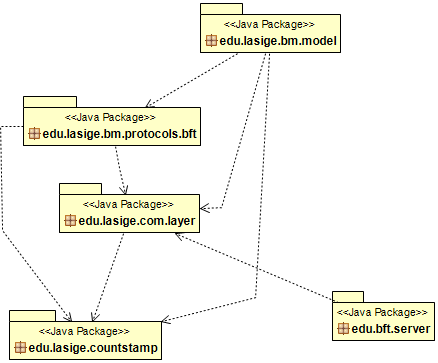
\includegraphics[width=0.7\textwidth]{class_diagram-minBFT.png}
\caption{Σχεδιάγραμμα των βασικών πακέτων του MinBFT.}
\label{fig:classdiagram}
\end{figure}

Το package \textbf{edu.lasige.com.layer} είναι υπεύθυνο για την επικοινωνία των διακομιστών και την διαχείρηση των μυνημάτων που λαμβάνει ο κάθε διακομιστής. Οι δύο βασικές κλάσεις μεσα στο πακέτο ειναι η $CommunicationSystem$ και η $BatchControl$. Η κλάση $CommunicationSystem$ αναλαμβάνει την λήψη και την μετάδοση των μυνημάτων, από και προς το $BatchControl$. Στην κλάση $BatchControl$ προωθείται καθε μήνυμα που λαμβάνει ο διακομιστής και ανάλογα με τον τύπο του μηνύματος κάνει τις αντίστοιχες λειτουργίες.

Η τεχνολογία Intel SGX στους υπολογιστές από προεπιλογή είναι απενεργοποιημένη. Για να χρησιμοποιήσει κανείς το Intel SGX πρέπει να το ενεργοποιήσει αρχικά μέσω του BIOS. Αυτό απαιτεί ένα BIOS όπου από τον κατασκευαστή του υποστηρίζει ρητά το Intel SGX. Η υποστήριξη που παρέχεται από το BIOS μπορεί να ποικίλει μεταξύ κατασκευαστών. Για να λειτουργήσει το Intel SGX, αφού ενεργοποιήσουμε στο BIOS, πρέπει να εγκατασταθεί στο σύστημα το πακέτο λογισμικού Intel SGX Platform (ή αλλιώς PSW)\cite{linuxsgx}. 

Η τεχνολογία Intel SGX στους υπολογιστές από προεπιλογή είναι απενεργοποιημένη. Για να χρησιμοποιήσει κανείς το Intel SGX πρέπει να το ενεργοποιήσει αρχικά μέσω του BIOS. Αυτό απαιτεί ένα BIOS όπου από τον κατασκευαστή του υποστηρίζει ρητά το Intel SGX. Η υποστήριξη που παρέχεται από το BIOS μπορεί να ποικίλει μεταξύ κατασκευαστών. Για να λειτουργήσει το Intel SGX, αφού ενεργοποιήσουμε στο BIOS, πρέπει να εγκατασταθεί στο σύστημα το πακέτο λογισμικού Intel SGX Platform (ή αλλιώς PSW)\cite{linuxsgx}. 

\section{Πώς τρέχει το MinBFT-SGX}
Η τεχνολογία Intel SGX στους υπολογιστές από προεπιλογή είναι απενεργοποιημένη. Για να χρησιμοποιήσει κανείς το Intel SGX πρέπει να το ενεργοποιήσει αρχικά μέσω του BIOS. Αυτό απαιτεί ένα BIOS όπου από τον κατασκευαστή του υποστηρίζει ρητά το Intel SGX. Η υποστήριξη που παρέχεται από το BIOS μπορεί να ποικίλει μεταξύ κατασκευαστών. Για να λειτουργήσει το Intel SGX, αφού ενεργοποιήσουμε στο BIOS, πρέπει να εγκατασταθεί στο σύστημα το πακέτο λογισμικού Intel SGX Platform (ή αλλιώς PSW)\cite{linuxsgx}. 
Αφού έχουμε κάνει όλα τα παραπάνω, εκτελούμαι την παρακάτω εντολή σε κάθε διακομιστή: 
\begin{lstlisting}[style=mystyle] 
java -cp dist/LASIGE-BFT-Protocols.jar:lib/* edu.bft.server.ServerCS [server id] [protocol] [size] [delay attack] [batchSize]
\end{lstlisting}
Το όρισμα $[server id]$ δηλώνει το αναγνωριστικό του διακομιστή, το $[protocol]$ είναι κάθε φορά MinBFT, το $[size]$ δηλώνει το μέγεθος του μηνύματος που στέλνει για απάντηση ο διακομιστής, στο $[delay attack]$ αν δώσουμε τιμή μεγαλύτερη από το 0 δηλώνει σε πόσο χρόνο αυτός ο διακομιστής θα καταρρεύσει και τέλος το $[batchSize]$ το οποίο δηλώνει πόσα μηνύματα θα επιβεβαιώνει ταυτόχρονα.

\section{Προγράμματα Αξιολόγησης (Benchmarks)} \label{benchmarksSection}
Η τεχνολογία Intel SGX στους υπολογιστές από προεπιλογή είναι απενεργοποιημένη. Για να χρησιμοποιήσει κανείς το Intel SGX πρέπει να το ενεργοποιήσει αρχικά μέσω του BIOS. Αυτό απαιτεί ένα BIOS όπου από τον κατασκευαστή του υποστηρίζει ρητά το Intel SGX. Η υποστήριξη που παρέχεται από το BIOS μπορεί να ποικίλει μεταξύ κατασκευαστών. Για να λειτουργήσει το Intel SGX, αφού ενεργοποιήσουμε στο BIOS, πρέπει να εγκατασταθεί στο σύστημα το πακέτο λογισμικού Intel SGX Platform (ή αλλιώς PSW)\cite{linuxsgx}. 

Η τεχνολογία Intel SGX στους υπολογιστές από προεπιλογή είναι απενεργοποιημένη. Για να χρησιμοποιήσει κανείς το Intel SGX πρέπει να το ενεργοποιήσει αρχικά μέσω του BIOS. Αυτό απαιτεί ένα BIOS όπου από τον κατασκευαστή του υποστηρίζει ρητά το Intel SGX. Η υποστήριξη που παρέχεται από το BIOS μπορεί να ποικίλει μεταξύ κατασκευαστών. Για να λειτουργήσει το Intel SGX, αφού ενεργοποιήσουμε στο BIOS, πρέπει να εγκατασταθεί στο σύστημα το πακέτο λογισμικού Intel SGX Platform (ή αλλιώς PSW)\cite{linuxsgx}. 

\begin{table}[h!]
\centering
\begin{tabular}{ | c | c | }
 \hline
 \multicolumn{2}{|c|}{Σύνοψη προγραμμάτων για benchmark} \\
 \hline
 Πρόγραμμα & Περιγραφή\\
 \hline
 SgxTimeTest &  \vtop{\hbox{\strut Υπολογισμός μέσης διάρκειας για την αύξηση }\hbox{\strut ενός μονοτονικού μετρητή με το Intel SGX }} \\ \hline
 ThroughputClient & Μέτρηση του throughput των διακομιστών  \\ 
 \hline
 ClientThread & Μέτρηση της μέσης καθυστέρησης για ένα σύνολο μηνυμάτων  \\ 
 \hline
 LatencyClient & Μέτρηση της μέσης καθυστέρησης για ένα μήνυμα\\
 \hline
\end{tabular}
\caption{Σύνοψη και περιγραφή των προγραμμάτων αξιολόγησης που χρησιμοποιήθηκαν}
\label{table:benchmarkprograms}
\end{table}


\subsection{Πώς τρέχουν οι clients}
Η τεχνολογία Intel SGX στους υπολογιστές από προεπιλογή είναι απενεργοποιημένη. Για να χρησιμοποιήσει κανείς το Intel SGX πρέπει να το ενεργοποιήσει αρχικά μέσω του BIOS. Αυτό απαιτεί ένα BIOS όπου από τον κατασκευαστή του υποστηρίζει ρητά το Intel SGX. Η υποστήριξη που παρέχεται από το BIOS μπορεί να ποικίλει μεταξύ κατασκευαστών. Για να λειτουργήσει το Intel SGX, αφού ενεργοποιήσουμε στο BIOS, πρέπει να εγκατασταθεί στο σύστημα το πακέτο λογισμικού Intel SGX Platform (ή αλλιώς PSW)\cite{linuxsgx}. 
\begin{lstlisting}[style=mystyle] 
java -cp dist/LASIGE-BFT-Protocols.jar:lib/* edu.bft.client.ThroughputClient [client id] [request] [concurrent] [interval]
\end{lstlisting}